\chapter{Experiments} \label{chap:experiments}

In this section, we will be introducing the experiment we are conducting as well as showcasing different steps we are undertaking in order to conduct our experiment among a few other things. For example, the background and summary for different kinds and types of web frameworks. Firstly, we will introduce the background leading to the experiment and the motivation behind the experiment. After that, we will list out our detailed goals, hypothesis and expectations from the experiment as well as our hardware and software environment configuration. Then, we will setup and start conducting the experiment while simultaneously explaining and justifying each of the steps during the process.

After the experiment, we will first collect all the data that was produced from the experiment. We will than start analysing and categorising the collected data, process them and present them in the "Result" section. Furthermore, we will provide our verdict of the experiment by delivering discussions on the experiment itself such as whether the result was largely within our expectation or perhaps the results differs from our initial assumption and prediction by a considerable margin.

Finally, we will list the challenges we faced and the irregularities we found during our experiment, as well as possible future work that might be worth undertaking in the "Discussion" section.

\bigskip
\section{Expending on the Experiment Background}

From the evaluation section above, we stated that during the framework benchmarking experiment, we expect the WebAssembly framework to come out on top from a variety of benefits it provides. Such as a lower computation overhead and better RTT delays.

Our experiment will first be conducted in a controlled environment. Depends on the result we receive from this stage of the experiment, we then decide what the next stage of our experiment will be. This can either be designing, implementing and to carry out a "real-life" scenario experiment with both frameworks, or to expend, understand and conduct further research into the potential irregularities observed within the collected data from the first stage of the experiment.

This way, we will be extra confident with the data we collected from the experiment. Therefore, we shall have a stronger argument when communicating our results and our findings to other researchers and engineers, as well as making sure that the results we get are as accurate as possible.

\bigskip
\textbf{{\Large Chapter 4.2 Motivation}}

We focused on edge computing a lot in this thesis, we understand that edge computing is getting more popular everyday. According to Google searches, we are about 4 times more interested in edge computing than we were just 5 years ago [34]. Large information systems and tech companies have also developed their own edge computing frameworks and products, such as Google with Firebase Cloud Functions [35], Cloudflare with Cloudflare workers [36] and Vercel - The creator for Next.js [37], one of the most popular web frameworks, recently entered the edge computing market by introducing edge function for the framework [39].

\bigskip
\begin{figure}[hp]
\centering
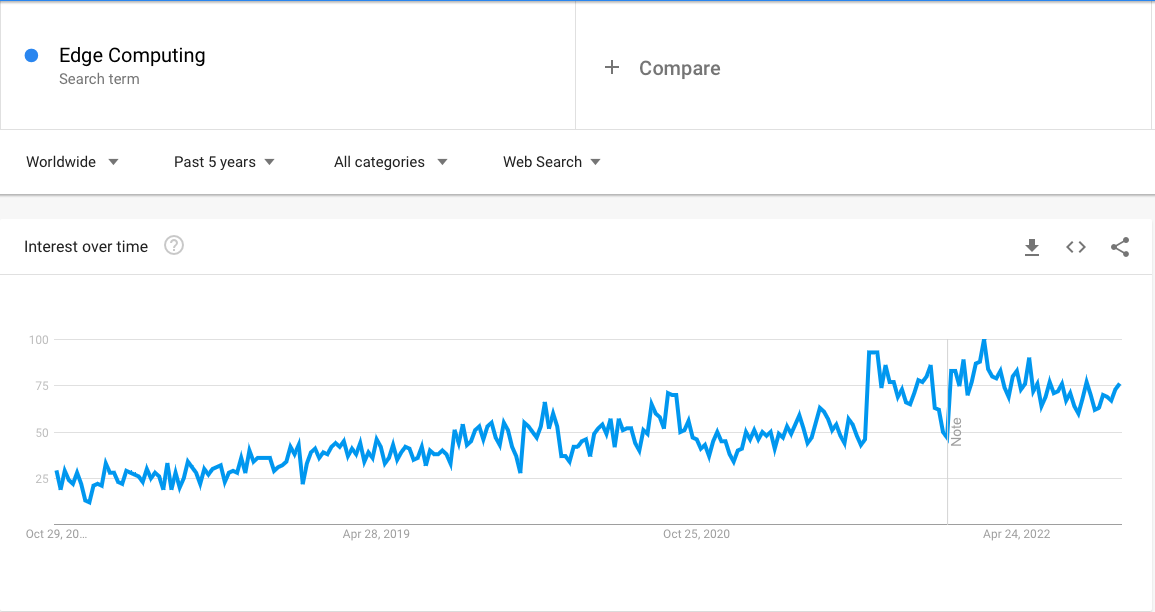
\includegraphics[scale=0.35]{edge-computing-trends}
\caption{\footnotesize{Google trends for edge computing}}
\captionsetup{aboveskip=0pt,font=it}
\end{figure}
\bigskip

However, with the current implementation, hosting server-side applications on the edge is just very inefficient. For example, according to Gadepalli et al. [39], the majority of the current implementation approach is either VM-Based (Virtual Machine) or Container-Based.

For VM-Based approach, each application are hosted in separate virtual machines within a physical hardware. Each virtual machine consists of its own operating system, kernel resource management, library dependencies and language runtimes. All of these resources will than be utilised to run the application deployed from the client. On the top level, the physical hardware usually known as a VM manager manages each of these virtual machines by distributing memory and CPU resources and over watching the processing thread. This approach is used by a number of well-known cloud service providers. For example, AWS Lambda and Azure Functions [40] [41].

Container-Based implementation uses a more straight forward structure than VM-Based implementation. With Container-Based implementation, each applications will be hosted in containers as per name suggested. Each containers also contains its own library dependencies as well as language runtimes. However, unlike the virtual machine approach, containers have direct access to the hardware's memory and CPU as well as limited access to certain system APIs. With this method, applications are no longer hosted in virtual machines, therefore it usually have a faster cold start latency than VM-Based approach. Popular services such as Google Cloud Function and Apache OpenWhisk uses this approach [42] [43].

After getting familiarised with the current technology, my natural research instinct kicked in, I kept asking myself if this is something that can be looked into and perhaps to be researched and experimented. From all the readings and literature reviews, it is easy to assume that WebAssembly simply has a better performance than the current technology including when running on the edge. However, we don't know the answer yet as this is only an assumption. Therefore, we are interested in comparing the performance between the two and we would like to conduct experiments in environments and scenarios described above.

\newpage
\begin{figure}[hp]
\centering
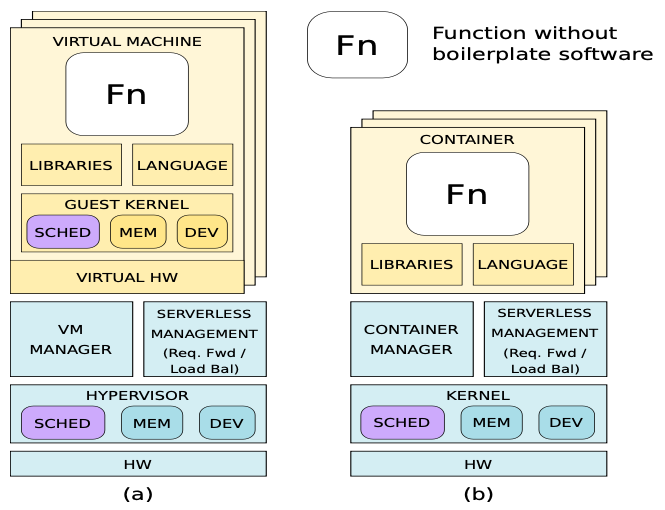
\includegraphics[scale=0.5]{sledge-design-a-b}
\caption{\footnotesize{Visualisation of the current edge computing system design layout, \textbf{a}: VM-Based implementation, \textbf{b}: Container-Based implementation}}
\captionsetup{aboveskip=0pt,font=it}
\end{figure}
\bigskip

\textbf{{\Large Chapter 4.3 Further Understanding on client-side application and server-side application}}

A web framework, sometimes also referred as a web application framework, is a collection of functionalities and libraries that is engineered and designed with the intention of laying the groundwork and providing basic infrastructures and logic for applications to be built on top of. This is so that developers and engineers working on the project do not have to implement such functionalities themselves. it simplifies the development process, reduces development time and increases development productivity output [44].

There are usually two categories of web frameworks: client-side framework and server-side framework. The former is usually used in order to construct dynamic web applications [45] while the latter is usually used to develop back-end API services. According to the 2022 annual developer survey from stack overflow [53], some of the most popular client-side frameworks including React.js [46], Angular [47] and Vue.js [48] while some of the most popular server-side frameworks including Node.js [49], ASP.NET [50] and Django [51] (server-side Django REST framework) [52].

It has been mentioned in multiple research articles that running full web applications using the current cloud solution may produce too much overhead, thus leads to inefficiency. For example, Gackstatter [54] recognise the limitation of today's "cloud-centric model" when it comes to deploying web applications at the edge. Specifically, the author stated that applying the current solution such as virtual machines and containers does not promise to be an effective solution due to limited resources available. Additionally, Gadepalli et al. not only pointed out the widely adoption of the virtual machine/container model, but also stated that server applications built using WASM functions that runs naively have the potential to expand the current use case of comprehensive applications running from the edge due to the reduction of the overhead which reduce the respond time down to within 10 milliseconds [39].

With the current model of implementation, Docker [77] and Kubernetes [78] are usually used in the publishing process in order to prepare an application for edge deployment. This would "wrap" the application into containers which will be further deployed onto self-managed serverless infrastructures or cloud computing service providers that provide edge services such as Amazon Web Service or Microsoft Azure. Those services will then distribute the application to edge devices across data centres around the world.

The topic and question of my research is to discover the performance gap and inconsistency between the current implementation of edge applications which includes application development and deployment with virtual machines, containers and traditional language runtimes, with the proposed WebAssembly solution which is to run functions as microservices directly from the native operating system using WebAssembly through a WASM runtime.

Currently at this stage, the true performance capability of WebAssembly has not yet been fully realised due to the relatively short time it has been around in comparison to JavaScript - which has almost 30 years of development. However, it is apparent to us that WebAssembly have a huge potential in terms of it's performance both when running in web browsers as well as running on operating systems naively through a runtime. We are able to back this up with the performance data of JavaScript over the years. In a presentation, Verschore presented a figure which stated that between 2001 and 2009, there was an 100-times improvement in JavaScript's performance as well as huge increases in the browser Octane score (web page loading speed) [55].

\newpage
\begin{figure}[!ht]
\centering
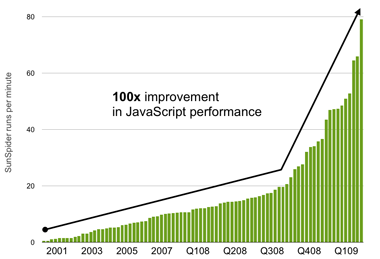
\includegraphics[scale=0.7]{js-perf}
\caption{\footnotesize{SunSpider benchmark score for the SpiderMonkey engine which is used in Firefox}}
\captionsetup{aboveskip=0pt,font=it}
\end{figure}

On top of that, the V8 JavaScript engine [58] behind popular browsers such as Google Chrome [56] and Brave [57], also had an incredible journey from when it was first released to the public back in 2008. The V8 development team undertook and released a set of benchmark scores comparing the performance of the Chrome browser from it's original beta to the versions in 2018. The results showed that in just 10 years, both its V8 Bench score [59] and Speedometer score [60] increased by 4 times, and the engine had also became a lot more stable as well as added support for a lot more chip architectures such as ARM and ARM 64 [61] [62].

\bigskip
\begin{figure}[hp]
\centering
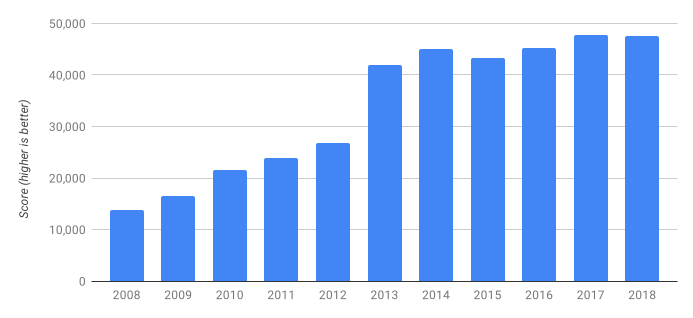
\includegraphics[scale=0.5]{chrome-v8-bench}
\caption{\footnotesize{Google Chrome's V8 Bench score between its original beta and the version in 2018}}
\captionsetup{aboveskip=0pt,font=it}
\end{figure}

\newpage
\begin{figure}[hp]
\centering
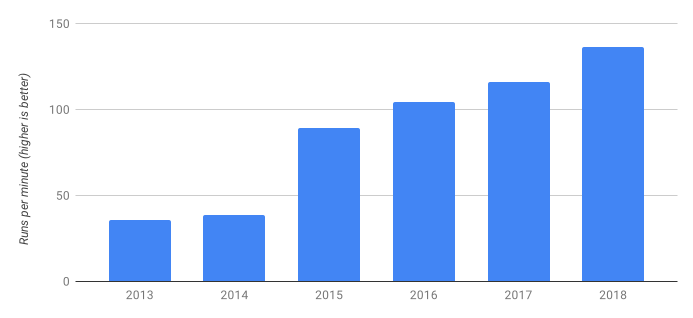
\includegraphics[scale=0.5]{chrome-speedometer-1}
\caption{\footnotesize{Google Chrome's Speedometer 1 score between its original beta and the version in 2018}}
\captionsetup{aboveskip=0pt,font=it}
\end{figure}
\bigskip

One of the recent example is the new Bun.js JavaScript runtime [79]. It is a newly released run time at the time of writing. It was build with the prior experience of Node.JS and made several visible improvements on top of that. Namely adding the support for edge computing.

\bigskip
\begin{figure}[hp]
\centering
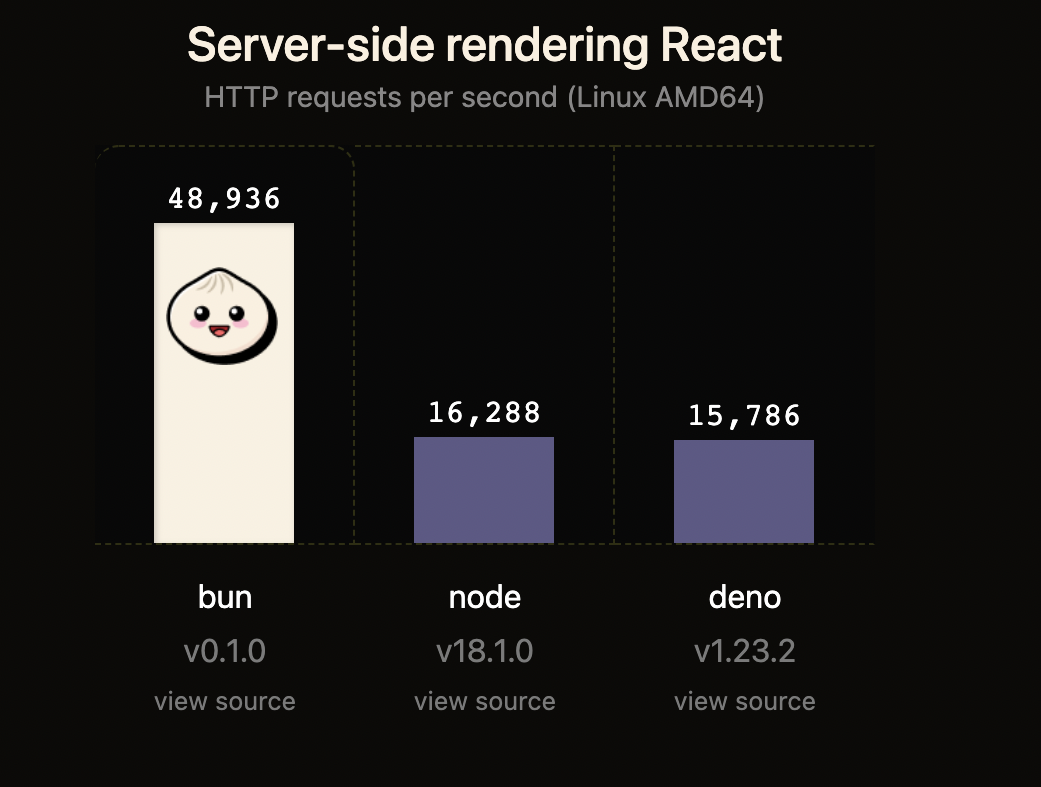
\includegraphics[scale=0.35]{bun-comparison}
\caption{\footnotesize{Performance comparison on HTTP requests between Bun and Node.JS}}
\captionsetup{aboveskip=0pt,font=it}
\end{figure}
\bigskip

\bigskip
\textbf{{\Large Chapter 4.4 WebAssembly framework options}}

Our experiment will focus on the two categories of microservice frameworks: VM/Container based frameworks and WebAssembly based frameworks. In addition, with each experiment scenarios, we will run it in our local environment as well as on the cloud computing server.

Here are some of the WebAssembly frameworks we are interested in. In this section, we will compare and analyse and in addition, to identify the strengths, weaknesses as well as characteristics for each of the frameworks. At the end, we will choose a framework that aligns with our interests the most.

\bigskip
\begin{table}[h!]
\centering
\begin{tabular}{||c c c||} 
\hline
Name & Developer & Website \\ [1ex] 
\hline\hline
 & & \\
Sledge & George Washington University & github.com/gwsystems/sledge-serverless-framework \\ 
 & & \\
Spin & Fermyon & github.com/fermyon/spin \\
 & & \\
WasmEdge (Runtime) & Linux foundation & wasmedge.org \\
 & & \\
Krustlet (Kubelet) & Deislabs & krustlet.dev \\
 & & \\
WAGI & Deislabs & github.com/deislabs/wagi \\
 & & \\
Wasmcloud & Wasmcloud team & wasmcloud.dev \\ [1ex]
\hline
\end{tabular}
\caption{List of WebAssembly frameworks of interest}
\label{table:webassembly_frameworks}
\end{table}

\bigskip
\textbf{{\normalsize Chapter 4.4.1 Sledge}}

Sledge framework was created and developed by the researchers at George Washington University. It offers a fast yet lightweight user experience and is designed to be run using WebAssembly runtimes natively. On top of that, the researchers have also developed a custom WASM runtime for it, called AWSM [80] (pronounced Awesome) using the Rust language [81]. However, both projects have yet to be production ready and are still in the testing phase. Adding on to that, they have yet to provide an official deployment instruction for the framework.

\bigskip
\textbf{{\normalsize Chapter 4.4.2 Spin}}

The Spin framework by the Fermyon company is one of the most popular server-side WebAssembly frameworks out there at the moment. It is also featured in multiple news articles including Yahoo! Finance [82] and Forbes [83]. Although not fully production ready yet, a considerable amount of testing have been done on the framework and the it has gained a considerable amount of attention within the backend server-side community.

On top of that, Fermyon has implemented and documented a detailed set of deployment instructions for spin. They created their own Platform-as-a-service solution - Fermyon cloud to host and manage Fermyon applications. They also teamed up with Deislabs which is another major company in the WebAssembly server-side market to deploy spin applications to Amazon Web Service through its Hippo bundler.

\bigskip
\textbf{{\normalsize Chapter 4.4.3 WAGI}}

WAGI is a product made by the aforementioned Deislabs. It is a super lightweight WebAssembly HTTP framework in its very early stage of development. WAGI is just like spin in many ways. It is able to compile the code down to WASM32-WASI which is a type of WebAssembly binary code. Therefore, it is able to run with any programming languages that compiles to WASM32-WASI, such as Rust and Go. However, unlike spin, it is only classified as experimental code and Deislabs currently does not have the plan to further develop WAGI into a production ready product. It also does not have an official deployment method.

\bigskip
\textbf{{\normalsize Chapter 4.4.4 Wasmcloud}}

Wasmcloud is a server-side backend framework and runtime that runs on all three major operating systems, Windows, macOS and Linux. On top of that, it is a polyglot platform which allows the same application being developed using multiple programming languages. In this case, AssemblyScript, Go or Rust. It was designed with security and scalability in mind. It also functions as an ecosystem where each functions are called "actors", Wasmcloud provides it's own Paas cloud computing service to deploy server-side applications, IoT applications as well as client-side applications running in web browsers. Furthermore, it has built-in edge support and has a detailed set of instruction and documentation on the deployment procedure.

\bigskip
\textbf{{\Large Chapter 4.5 Decision on Frameworks and Environment }}

We start by choosing a WebAssembly framework. We looked at the properties of the WebAssembly frameworks above and we decided to go with Spin by Fermyon. There are a few reasons contributing to this decision. Spin has a very detailed set of documentation as well as example projects. More crucially, there exists a research gap here as there hasn't been any tests performed on spin running on the edge.

On the other hand, the other non-WebAssembly traditional framework we will be utilising into our experiment is Flask [52]. As stated above, Flask is a Python HTTP microservice framework. It is currently one of the most popular traditional non-Webassembly frameworks and Python is also one of the most popular programming language.

The local environment for conducting our experiments will be on a 2017 MacBook Pro running with the Intel Core I5-7267U CPU (2 cores, 3.1 GHz), it has an 8GB memory with 512GB internal SSD storage. For the production environment, we will be using Amazon Web Service for our cloud and edge deployment. Specifically, we will be utilising the Amazon EC2 service to host our applications [87]. Amazon EC2 offers a wide range of instances (server computers) that suits the need for most businesses ranging from small IoT controller computers to large industrial servers for server farms [88]. In our case, both of our frameworks will be deployed and run on an AWS t3 micro instance. The t3 micro instance is a medium rage server. It has 2 vCPUs (Intel Xeon or AMD EPYC, both running up to 3.1 GHz) with 1GB memory and on-demand elastic storage (it charge its customers based on the amount of storage it holds). It is designed to run applications such as microservices, small to medium databases, business critical applications and so on [89]. It is small yet agile enough to be used as an edge server for our spin application, but also powerful enough to host our flask application for it to run in a traditional cloud environment.

\bigskip
\textbf{{\Large Chapter 4.6 Roadblocks in Early Stage of Experiment}}

The initial experiment plan is very distinct from the plan described in this section. In the early stage of carrying out the experiment, we planned to integrated PolyBench/C into our benchmarking experiment [93]. PolyBench is one of the best system benchmarking frameworks at the moment and it is originally written in C and the Fortran language by Louis-Noel Pouchet at The Ohio State University [94]. At first, we looked into benchmarking both of our frameworks with PolyBench/Python [95]. Which is a re-implementation of the original PolyBench/C developed by Abella-Gonzalez et al. at the University of A Coruna in Spain alongside with Louis-Noel Pouchet himself. However, when browsing through the project code, we discovered that PolyBench/Python is only available for x86 architecture machines running with Linux due to a number of runtime dependencies only available on the Linux operating system. We initially do not have access to such machines but we later installed a copy of Ubuntu Linux operating system as a virtual machine through Oracle VM VirtualBox [96] [97]. However, at the end, we decided that we won't go ahead with PolyBench/Python due to the potential system compatibility issues we might have on deployment. Therefore, we continued our experiment with the original PolyBench/C framework.

\bigskip
\begin{figure}[hp]
\centering
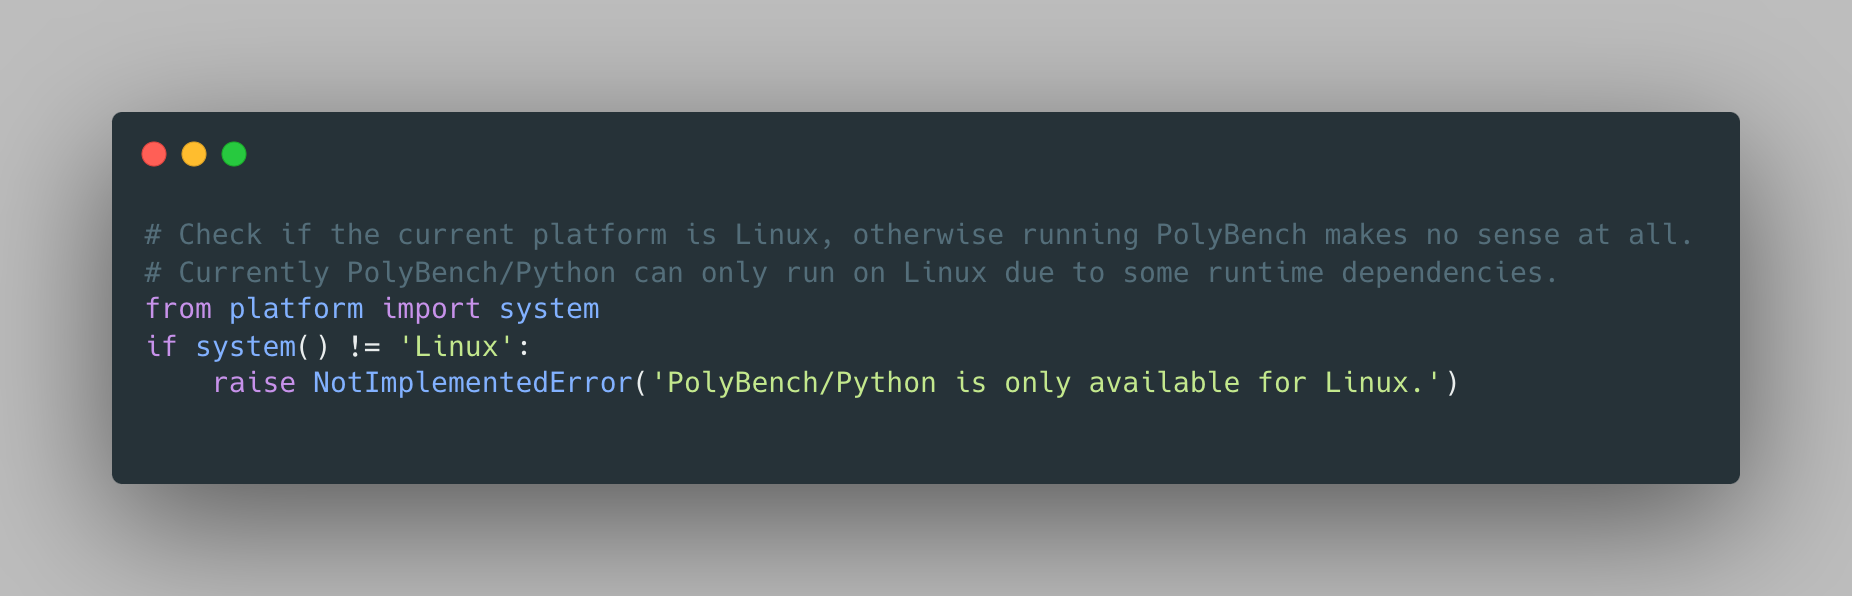
\includegraphics[scale=0.24]{polybench-python}
\caption{\footnotesize{Code snippet on PolyBench/Python compatibility}}
\captionsetup{aboveskip=0pt,font=it}
\end{figure}
\bigskip

There are 30 benchmarking tests in PolyBench/C, its operation covers the majority of everyday computing tasks. PolyBench/C includes numerical computations extracted from various applications. This includes: linear algebra, image processing, physics simulation, dynamic programming, statistics and so on. Each benchmark tests includes a single C program file along with its header H file. User runs the benchmark file by first compiling it to a UNIX executable file with a C compiler such as gcc or clang [98] [99]. After that, they can then generate the output of the program by running it in a terminal application as well as passing in the desired name of the output file. Users can also pass in extra configuration options to alter the compilation process as well as the desired output. For example, to display the program execution time or to change the input dataset size.

The source code of the project can be found here: \href{https://web.cse.ohio-state.edu/~pouchet.2/software/polybench/}{\color{blue}{The Polyhedral Benchmark Suite}}. Here is a list of all benchmark tests (Version 4.2.1) and their descriptions:

\bigskip
\begin{table}[h!]
\centering
\begin{tabular}{||c c||} 
\hline
Name & Description \\ [1ex] 
\hline\hline
 & \\
2mm & 2 Matrix Multiplications (alpha * A * B * C + beta * D) \\ 
 & \\
3mm & 3 Matrix Multiplications ((A*B)*(C*D)) \\ 
 & \\
adi & Alternating Direction Implicit solver \\ 
 & \\
atax & Matrix Transpose and Vector Multiplication \\ 
 & \\
bicg & BiCG Sub Kernel of BiCGStab Linear Solver \\ 
 & \\
cholesky & Cholesky Decomposition \\ 
 & \\
correlation & Correlation Computation \\ 
 & \\
covariance & Covariance Computation \\ 
 & \\
deriche & Edge detection filter \\ 
 & \\
doitgen & Multi-resolution analysis kernel (MADNESS) \\ 
 & \\
durbin & Dynamic programming (2D) \\ 
 & \\
dynprog & Toeplitz system solver \\ 
 & \\
fdtd-2d & 2-D Finite Different Time Domain Kernel \\ 
 & \\
gemm & Matrix-multiply C=alpha.A.B+beta.C \\ 
 & \\
gemver & Vector Multiplication and Matrix Addition \\ 
 & \\
gesummv & Scalar, Vector and Matrix Multiplication \\ [1ex]
\hline
\end{tabular}
\caption{PolyBench/C Benchmarks}
\label{table:time_complexity_2}
\end{table}

\begin{table}[h!]
\centering
\begin{tabular}{||c c||} 
\hline
Name & Description \\ [1ex] 
\hline\hline
 & \\
gramschmidt & Gram-Schmidt decomposition \\ 
 & \\
head-3d & Heat equation over 3D data domain \\ 
 & \\
jacobi-1D & 1-D Jacobi stencil computation \\ 
 & \\
jacobi-2D & 2-D Jacobi stencil computation \\ 
 & \\
lu & LU decomposition \\ 
 & \\
ludcmp & LU decomposition followed by Forward Substitution \\ 
 & \\
mvt & Matrix Vector Product and Transpose \\ 
 & \\
nussinov & Dynamic programming algorithm for sequence alignment \\ 
 & \\
seidel & 2-D Seidel stencil computation \\ 
 & \\
symm & Symmetric matrix-multiply \\ 
 & \\
syr2k & Symmetric rank-2k update \\ 
 & \\
syrk & Symmetric rank-k update \\ 
 & \\
trisolv & Triangular solver \\ 
 & \\
trmm & Triangular matrix-multiply \\ [1ex]
\hline
\end{tabular}
\caption{PolyBench/C Benchmarks (continued 1)}
\label{table:time_complexity_2}
\end{table}

We continue our experiment by start utilising the PolyBench/C code. We designed a program that compiles and execute all 30 algorithms with 5 difference set of data sizes: mini, small, medium, large and extra large.

The program will first construct a list of relevant paths of all benchmark files from the pre set dictionary of \mintinline{python}{ALL_FILES}. After that, the program will create an temporary folder in the project root directory called \mintinline{python}{compiled}, it will then compile all benchmarks into compiled UNIX executable binary files using the gcc compiler and store them into the \mintinline{python}{compiled} folder. For each benchmarks, after its compiled, we will run the program with the 5 aforementioned datasets. After running the binary executable files, we can output and log their runtimes. We do this by writing them in a text file with the naming convention (see below) and saving it persistently in a folder named \mintinline{python}{results} also in the project root directory. Finally after all results were collected, we clean up the runtime environment by removing the \mintinline{python}{compiled} folder.

Result file naming convention:
\newline
\mintinline{python}{output-file-<current date and time (Day-Month-Year-Hour-Minute-Second)>.txt}

The program source code is available publicly on GitHub.
\newline
The link can be found \href{https://github.com/richard875/Honours-PolyBench}{\color{blue}{here (GitHub: richard875/Honours-PolyBench)}}

After developing the PolyBench testing project, we are ready to integrate it with our testing frameworks. The PolyBench testing project was designed to be used as a "module". We achieve this by implementing and exposing a \mintinline{python}{main} function that can be called externally and returns the runtime benchmark data.

We first integrate it with the flask framework, we develop and configure the project so that it calls the \mintinline{python}{main} function on receiving a connection on a particular route, in this case the index \mintinline{python}{/} route, then return and display the timing data on render.

We then integrate it with the spin WebAssembly framework. We did largely the same with the flask framework. We also point the index route to execute the \mintinline{python}{main} function. However, this time the program failed to execute and the benchmarks did not compile.

After conducting further research, we found that it is an expected behaviour for WebAssembly frameworks. As stated in the literature review section, one of the main benefits of WebAssembly is its security. WebAssembly applications executes in a sandboxed environment that is separated from the host environment and only expose limited APIs that was proven to be safe for developers to use [100]. Therefore, in a WebAssembly environment, code such as \mintinline{python}{os.path.isdir(RUNTIME_OUTPUT_FOLDER)} which checks if a directory exists or \mintinline{python}{shutil.rmtree(RUNTIME_OUTPUT_FOLDER, ignore_errors=True)} which deletes a directory folder along with all its contents will not work.

Therefore, we had to stop pursuing this experiment path and change our experiment direction.

\bigskip
\textbf{{\Large Chapter 4.7 Initial Dataset}}

After the previous roadblock, we started to look for other benchmarking solutions. After further researches, we decided that we will start the experiment with a custom collection of sorting algorithms. Some of the most popular sorting algorithms out there including Bubble sort [84], Insertion sort [85] and Quick sort [86]. Sorting algorithms are an excellent way to benchmark the runtime for individual web frameworks as they don't require any incoming or outgoing connections and thus do not have any external uncontrollable factors. Unlike PolyBench, they do not need to be compiled into as standalone files to be run. Furthermore, sorting algorithms are also available in multiple languages (we will use Python in our case). As such, they can be run in almost any environments.

During our experiment, we found that it is very difficult to come up with a set of "one-fits-all" number list input. For instance, some sorting algorithms in our collection take massively longer to complete than others.

We define our list input size (number of elements in the input list) as \(N\). We than set \(N = 1000\) and run the algorithm in local environment. Faster sorting algorithms such as Quick sort and Merge sort took 0.002s and 0.004s to run respectively, while slower sorting algorithms such as Gnome sort and Brick sort took 0.123s and 11.171s respectively (tested under local environment).

Here is a list of 18 sorting algorithms in our collection with their runtime boundary notation:

\bigskip
\begin{table}[h!]
\centering
\begin{tabular}{||c c c c||} 
\hline
Name & Best (Time) & Average (Time) & Worst (Time) \\ [1ex] 
\hline\hline
 & & & \\
Bitonic Sort & \(\Theta(log^2(n))\) & \(O(log^2(n))\) & \(\Omega(nlog^2(n))\) \\ 
 & & & \\
Bubble Sort & \(\Theta(n)\) & \(O(n^2)\) & \(\Omega(n^2)\) \\ 
 & & & \\
Brick/Odd-even Sort & \(\Theta(n)\) & \(O(n^2)\) & \(\Omega(n^2)\) \\ 
 & & & \\
Bucket Sort & \(\Theta(n)\) & \(O(n+\dfrac{n^2}{k}+k)\), \(k\) is number of buckets & \(\Omega(n^2)\) \\ 
 & & & \\
Cocktail Sort & \(\Theta(n)\) & \(O(n^2)\) & \(\Omega(n^2)\) \\ 
 & & & \\
Comb Sort & \(\Theta(nlog(n))\) & \(O(\dfrac{n^2}{2^p})\), \(p\) is number of increments & \(\Omega(n^2)\) \\ 
 & & & \\
Gnome Sort & \(\Theta(n)\) & \(O(n^2)\) & \(\Omega(n^2)\) \\ 
 & & & \\
Heap Sort & \(\Theta(nlog(n))\) & \(O(nlog(n))\) & \(\Omega(nlog(n))\) \\ 
 & & & \\
Insertion Sort & \(\Theta(n)\) & \(O(n^2)\) & \(\Omega(n^2)\) \\ 
 & & & \\
Merge Sort & \(\Theta(nlog(n))\) & \(O(nlog(n))\) & \(\Omega(nlog(n))\) \\ 
 & & & \\
Pancake Sort & \(\Theta(n)\) & \(O(n^2)\) & \(\Omega(n^2)\) \\
 & & & \\
Pigeonhole Sort & \(\Theta(N+n)\) & \(O(N+n)\) & \(\Omega(N+n)\), \(N\) is key value range \\ 
 & & & \\
Quick Sort & \(\Theta(nlog(n))\) & \(O(nlog(n))\) & \(\Omega(n^2)\) \\ 
 & & & \\
Radix Sort & \(\Theta(nk)\) & \(O(nk)\) & \(\Omega(nk)\), \(k\) is key length \\  [1ex]
\hline
\end{tabular}
\caption{Time complexity of sorting algorithms}
\label{table:time_complexity_1}
\end{table}

\begin{table}[h!]
\centering
\begin{tabular}{||c c c c||} 
\hline
Name & Best (Time) & Average (Time) & Worst (Time) \\ [1ex] 
\hline\hline
 & & & \\
Selection Sort & \(\Theta(n^2)\) & \(O(n^2)\) & \(\Omega(n^2)\) \\ 
 & & & \\
Shell Sort & \(\Theta(nlog(n))\) & depends & \(\Omega(n^2)\) \\ 
 & & & \\
Smooth Sort & \(\Theta(n)\) & \(O(nlog(n))\) & \(\Omega(nlog(n))\) \\ 
 & & & \\
Strand Sort & \(\Theta(n)\) & \(O(n^2)\) & \(\Omega(n^2)\) \\ [1ex]
\hline
\end{tabular}
\caption{Time complexity of sorting algorithms (continued)}
\label{table:time_complexity_2}
\end{table}
\bigskip

\bigskip
\textbf{{\Large Chapter 4.8 First Stage: Sorting Algorithm Development}}

We are now ready to start carrying out the experiment. The first stage of our experiment is to design and develop the algorithm collection. In this step, we gathered all 18 different algorithms of our choice. We collected the algorithm code from websites such as \href{https://www.geeksforgeeks.org/}{\color{blue}{geeksforgeeks.org}} and \href{https://www.programiz.com/}{\color{blue}{programiz.com}}. After that, we performed local tests on each of the algorithm functions to ensure that they are able to produce their desired outcome.

Each algorithm is essentially its own file, as stated above, the algorithms does not produce any outgoing traffic connections and it also doesn't have any import modules as we would like to keep uncontrolled factors to a minimum. Therefore, they are stand along code that can be executed on any platforms. We also implemented \mintinline{python}{if __name__ == "__main__":} module code in the algorithm files to prevent the code from being executed upon importation.

After all the algorithms are packaged and tested, we grouped all files into a folder to be used as a module. And then, we created our testing files to run and measure the time for each algorithm.

In our testing file, we imported all the algorithms from the above folder to be used during measurement. Furthermore, we will be using the Python \mintinline{python}{time} and \mintinline{python}{random} modules. At the beginning of the testing script, we constructed the arrays to be performed on. We do this by generating a number between 0 and \(N\), where \(N\) is either a fixed parameter defined within the script or passed in during runtime. For each array, we run this process \(L\) times, where \(L\) is the length of the array. In this case, \(N = L\).

As stated above, difference sorting algorithms have significant differences in performance and runtime. Therefore, it is difficult at best and almost impossible at worst to come up with a "one-for-all" array length to test the benchmarks for all sorting algorithms. This can be observed in Bingmann's 2013 article "The Sound of Sorting" [90]. In the article and the subsequent video [91], different algorithms are given different input length to achieve a similar runtime. For example, selection sort and quick sort both completed sorting in similar timeframes. However, selection sort only had an array input size of 130, yet quick sort has an array input size of 1440. The GitHub repository for the project can be found here [92]. Our solution to this is to perform tests locally with different input sizes to get a rough estimate on the time complexly for each algorithms. In the experiment, we will run each algorithm 5 times with 3 input array sizes - \mintinline{python}{small}, \mintinline{python}{medium} and \mintinline{python}{large}. In our local tests, we set our \mintinline{python}{small} input size to be run within around \mintinline{python}{2} seconds, \mintinline{python}{medium} input size to be run within around \mintinline{python}{5} seconds and \mintinline{python}{large} input size to be run within around \mintinline{python}{10} seconds. This is the performance benchmark we observed when running locally, however, we are fully expecting a drop in performance for both frameworks when running remotely in production due to various overheads as well as the increased physical distance between the client and the server.

Here is a list of detailed array input sizes \(N\) for each sorting algorithms:
\begin{table}[h!]
\centering
\begin{tabular}{||c c c c||} 
\hline
Name & Small & Medium & Large \\ [1ex] 
\hline\hline
 & & & \\
Bitonic Sort & 100000 & 200000 & 300000 \\ 
 & & & \\
Bubble Sort & 5000 & 7000 & 10000 \\ 
 & & & \\
Brick/Odd-even Sort & 600 & 800 & 1000 \\ 
 & & & \\
Bucket Sort & 35000 & 55000 & 70000 \\ 
 & & & \\
Cocktail Sort & 4000000 & 10000000 & 17000000 \\ 
 & & & \\
Comb Sort & 250000 & 550000 & 850000 \\ 
 & & & \\
Gnome Sort & 4000 & 6500 & 9000 \\ 
 & & & \\
Heap Sort & 200000 & 500000 & 900000 \\ 
 & & & \\
Insertion Sort & 6000 & 10000 & 14000 \\ 
 & & & \\
Merge Sort & 300000 & 700000 & 1400000 \\ [1ex]
\hline
\end{tabular}
\caption{Array input sizes for sorting algorithms}
\label{table:time_complexity_1}
\end{table}

\begin{table}[h!]
\centering
\begin{tabular}{||c c c c||} 
\hline
Name & Small & Medium & Large \\ [1ex] 
\hline\hline
 & & & \\
Pancake Sort & 4500 & 7000 & 10000 \\
 & & & \\
Pigeonhole Sort & 4000000 & 11000000 & 20000000 \\ 
 & & & \\
Quick Sort & 550000 & 1250000 & 2500000 \\ 
 & & & \\
Radix Sort & 450000 & 980000 & 1500000 \\
 & & & \\
Selection Sort & 6000 & 9500 & 14000 \\ 
 & & & \\
Shell Sort & 190000 & 400000 & 700000 \\ 
 & & & \\
Smooth Sort & 85000 & 200000 & 400000 \\ 
 & & & \\
Strand Sort & 20000 & 30000 & 35000 \\ [1ex]
\hline
\end{tabular}
\caption{Array input sizes for sorting algorithms (continued)}
\label{table:time_complexity_2}
\end{table}
\bigskip

\bigskip
\textbf{{\Large Chapter 4.9 Framework Deployment}}

Amazon Web Service (AWS) provides an excellent Paas platform for us to deploy both applications. We used services including Amazon ec2, Amazon Elastic Container Registry (ECR) and Amazon Elastic Container Service (ECS) [101] [102].

We containerised both applications into Docker containers, we do this by adding a \mintinline{python}{Dockerfile} file in the root of our project. Both applications use Ubuntu as the Docker container base image [103].

For our Flask application, we install \mintinline{python}{python3-pip}, as well as \mintinline{python}{Flask}. We then copy all files into the Docker container, finally starts the application in the Docker container by running the\newline\mintinline{python}{python3 -m flask run --host=0.0.0.0} command. We use \mintinline{python}{--host=0.0.0.0} to host the application on the server's public IPv4 address to be accessible on port 5000.

For our Spin application, we need to install the spin runtime provided by Fermyon from a bash script [104]. However, before that, we first need to install all dependencies needed to run the script. These are: \mintinline{python}{curl}, \mintinline{python}{build-essential}, \mintinline{python}{libssl-dev} and \mintinline{python}{pkg-config}. After that, we install the spin runtime binary by running the \mintinline{python}{install.sh} script. Finally, we start the application by running the \newline\mintinline{python}{./docker/spin up --listen 0.0.0.0:3000} command.

We upload our applications to AWS, both on ec2 services. However, with our spin application,
we will be using the Amazon CloudFront service to distribute the application to edge servers around the world [105]. Here is a list of cities with CloudFront edge servers and the number of edge locations within that city [106] [107]:

\begin{itemize}
   \item United States, Canada and Mexico
   \begin{itemize}
     \item Washington, DC (11)
     \item Chicago, IL (19)
     \item New York, NY (10)
     \item Atlanta, GA (10)
     \item Los Angeles, CA (9)
     \item Miami, FL (11)
     \item Dallas-Fort Worth, TX (11)
     \item Houston, TX (4)
     \item San Francisco, CA (6)
     \item Boston, MA (5)
     \item Denver, CO (3)
     \item Portland, OR (2)
     \item Seattle, WA (6)
     \item Toronto, ON (3)
     \item Minneapolis, MN (4)
     \item Phoenix, AZ (2)
     \item Querétaro, QT (2)
     \item Montréal, QC (2)
     \item Philadelphia, PA (1)
     \item Salt Lake City, UT (1)
     \item Vancouver, BC (1)
     \item Nashville, TN (2)
     \item Detroit, MI (2)
   \end{itemize}
   \item Europe
   \begin{itemize}
     \item Frankfurt (17)
     \item London (24)
     \item Paris (9)
     \item Milan (9)
     \item Rome (6)
     \item Berlin (5)
     \item Madrid (4)
     \item Marseille (4)
     \item Amsterdam (4)
     \item Düsseldorf (4)
     \item Hamburg (3)
     \item Manchester (5)
     \item Munich (4)
     \item Vienna (3)
     \item Stockholm (3)
     \item Copenhagen (2)
     \item Dublin (2)
     \item Helsinki (3)
     \item Athens (1)
     \item Brussels (1)
     \item Budapest (1)
     \item Lisbon (1)
     \item Oslo (2)
     \item Bucharest (1)
     \item Palermo (1)
     \item Prague (1)
     \item Sofia (1)
     \item Warsaw (1)
     \item Zagreb (1)
     \item Zurich (1)
   \end{itemize}
   \item Asia
   \begin{itemize}
     \item Tokyo (20)
     \item New Delhi (7)
     \item Seoul (6)
     \item Chennai (7)
     \item Singapore (6)
     \item Osaka (7)
     \item Mumbai (10)
     \item Bangalore (4)
     \item Hyderabad (3)
     \item Hong Kong (4)
     \item Taipei (3)
     \item Bangkok (10)
     \item Kolkata (2)
     \item Jakarta (2)
     \item Kuala Lumpur (2)
     \item Shanghai (1)
     \item Beijing (1)
     \item Shenzhen (1)
     \item Zhongwei (1)
     \item Manila (1)
     \item Hanoi (1)
     \item Ho Chi Minh City (1)
   \end{itemize}
   \item Australia and New Zealand
   \begin{itemize}
     \item Sydney, NSW (6)
     \item Auckland, NZ (3)
     \item Melbourne, VIC (2)
     \item Perth, WA (1)
   \end{itemize}
   \item South America
   \begin{itemize}
     \item São Paulo (7)
     \item Rio De Janeiro (2)
     \item Bogota (2)
     \item Buenos Aires (2)
     \item Santiago (1)
   \end{itemize}
   \item Middle East
   \begin{itemize}
     \item Tel Aviv (2)
     \item Manama (2)
     \item Dubai (1)
     \item Fujairah (1)
   \end{itemize}
   \item Africa
   \begin{itemize}
     \item Cape Town (1)
     \item Johannesburg (1)
     \item Nairobi (1)
   \end{itemize}
\end{itemize}
 
\bigskip
\textbf{{\Large Chapter 4.10 Second Stage: Dijkstra, Floyd, Kruskal and Prim}}

We conducted the first stage of our experiment. And we listed the detailed data in the Results section. To our surprise, and in contradictory to the initial hypothesis which suggested that Spin WebAssembly framework will perform better, we observed the opposite. On average, across all tests and benchmarks, Flask out performed Spin by \textbf{140\%} on average.

Based on the result from the first stage of the experiment, we decide to continue and expand on benchmarking our frameworks. By this stage of the experiment, we are able to recognise that Flask performs better than Spin. But we would like to discover if there are any differences between the performance gap for both frameworks running different kinds of algorithms (non-sorting algorithms). Therefore, we further introduced 4 algorithms: Dijkstra's algorithm, Floyd–Warshall algorithm, Kruskal's algorithm and Prim's algorithm. Similar to sorting algorithms, we will run each each algorithms 5 times inputting 3 set of datasets with different sizes.

\bigskip
\textbf{{\normalsize Chapter 4.10.1 Dijkstra's Algorithm}}

We use Dijkstra's Algorithm to find the shortest distance between two points on a map in practice. However, we usually represent this by finding the shortest path between two vertices in a graph [108]. In our benchmarking test, we set \(V\) to the number of vertices on a side with the total number of vertices being \(V^2\). Furthermore, each vertices are connected by an edge with a weight (distance) randomly generated between 0 and 20.

We run the algorithm on every single pair of vertices, which totals to \(V(V-1)/2\) pairs. The average runtime complexity is \(O(E+V\cdot\ Log(V))\) where \(E\) is the number of edges in the graph and \(V\) is the number of vertices in the graph. The size of the input datasets (number of edges) are 2500, 4000 and 5800 respectively. Thus, the total runtime for our Dijkstra's Algorithm benchmarking test is:

\[ O(V(V-1)/2 \cdot (E+V\cdot\ Log(V))\ where\ V \in \{2500, 4000, 5800\}, V = E \]

\bigskip
\textbf{{\normalsize Chapter 4.10.2 Floyd–Warshall Algorithm}}

The Floyd–Warshall Algorithm, also called Floyd's Algorithm, is a non-greedy shortest path algorithm [109]. However, unlike Dijkstra's Algorithm, Floyd–Warshall Algorithm does not work on graphs with negative cycles. In our benchmarking test, we set \(V\) to the number of vertices on a side with the total number of vertices being \(V^2\). We then set \(E\) to be the number of all edges in the graph where \(V = E\). Each edges have a 50\% chance of having an infinite weight. When this occurs, we consider the pair of vertices not connected. For connected edges, each has a weight distance randomly generated between 0 and 20.

We then run the algorithm on every single pair of vertices, which totals to \(V(V-1)/2\) pairs. The average runtime complexity is \(O(V^3)\) where \(V\) is the number of vertices in the graph. The size of the input datasets (number of edges) are 180, 250 and 310 respectively. Thus, the total runtime for our Floyd’s Algorithm benchmarking test is:

\[ O(V(V-1)/2 \cdot V^3) \]
\[ =O(V^4(V-1)/2)\ where\ V \in \{180, 250, 310\}  \]

Note: We observed that Floyd's Algorithm has a greater runtime complexity than Dijkstra's Algorithm. Thus, in order to keep the runtime similar, we reduced the input sizes for Floyd's Algorithm.

\bigskip
\textbf{{\normalsize Chapter 4.10.3 Kruskal's Algorithm}}

Kruskal's Algorithm is a greedy, minimum spanning tree algorithm [110]. A minimum spanning tree returns a list of edges where the sum of their weights are as small as possible [111].

\newpage
\begin{figure}[hp]
\centering
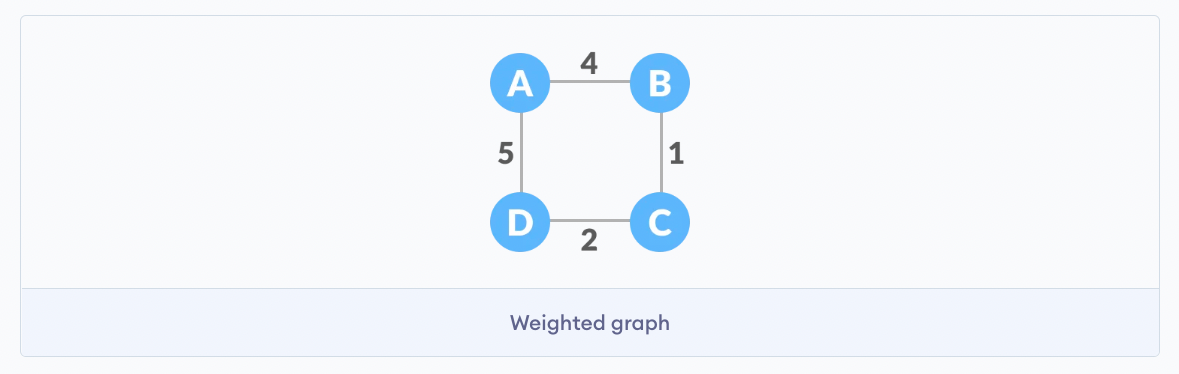
\includegraphics[scale=0.4]{minimum-spanning-tree-1}
\caption{\footnotesize{A Weighted Undirected Graph}}
\captionsetup{aboveskip=0pt,font=it}
\end{figure}
\bigskip

\begin{figure}[hp]
\centering
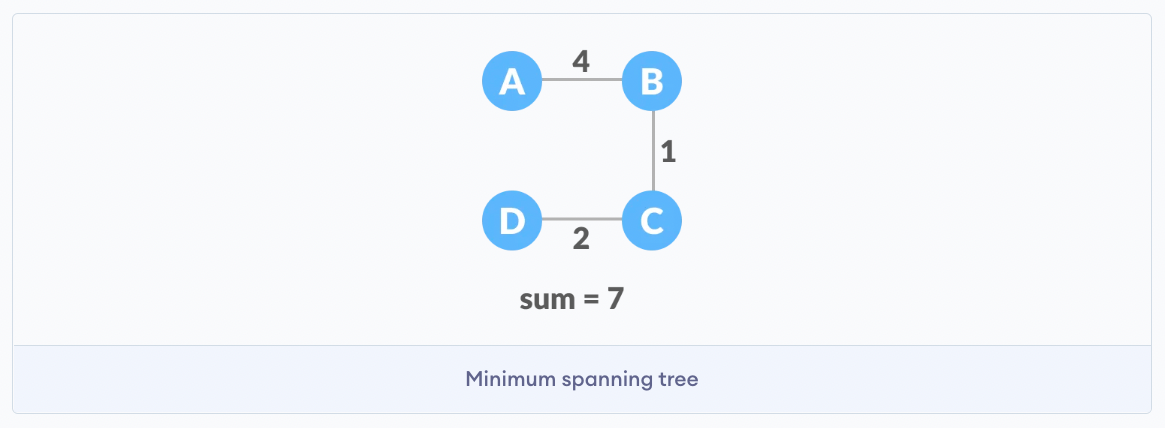
\includegraphics[scale=0.4]{minimum-spanning-tree-2}
\caption{\footnotesize{Minimum Spanning Tree for the above Graph, in this case 7 (4 + 1 + 2)}}
\captionsetup{aboveskip=0pt,font=it}
\end{figure}
\bigskip

In our testing script, we again set \(V\) to the number of vertices on a side with the total number of vertices being \(V^2\). Furthermore, we define \(E\) as edge, where \(E = V - 1\). Each \(E\) connects \(V[i]\) with \(V[i+1]\), where \(i\) is the index of \(E\).

We then run the algorithm on the graph and measure its runtime. The algorithm finds and traverses through the minimum spanning tree of our graph. The average runtime complexity is \(O(E\cdot\ Log(E))\) where \(E\) is the the total number of edges in the graph. The size of the input datasets (number of edges) are 400000, 1000000 and 2100000 respectively. Thus, the total runtime for our Kruskal’s Algorithm benchmarking test is:

\[ O(E\cdot\ Log(E))\ where\ E = V - 1, V \in \{400000, 1000000, 2100000\} \]
\[ =O(E\cdot\ Log(E))\ where\ E \in \{399999, 999999, 2099999\} \]

\bigskip
\textbf{{\normalsize Chapter 4.10.4 Prim's Algorithm}}

Finally, we benchmark Prim's Algorithm. Just like Kruskal’s Algorithm, Prim's Algorithm is a greedy, minimum spanning tree algorithm [112]. However, unlike Kruskal’s Algorithm, Prim's Algorithm selects the root vertex upon execution and gradually expand outwards until it has traversed the whole graph [113]. In our benchmarking test, we set \(V\) to be the number of vertices on a side with the total number of vertices being \(V^2\). After that, just like Floyd’s Algorithm, we set \(E\) to be the number of all edges in the graph where \(V = E\). Each edges have a 50\% chance of having an zero (0) weight. When this occurs, we consider the pair of vertices not connected. For connected edges, each has a weight distance randomly generated between 1 and 99.

We then run the algorithm on the graph and measure its runtime. Prim's Algorithm finds and traverses through the minimum spanning tree of our graph. Its average runtime complexity is \(O(E\cdot\ Log(V))\) where \(V\) is the number of vertices in the graph and \(E\) is the number of edges in the graph. The size of the input datasets (number of edges) are 400, 550 and 680 respectively. Thus, the total runtime for our Prim’s Algorithm benchmarking test is:

\[ O(E\cdot\ Log(V))\ where\ E, V \in \{400, 550, 680\} \]

\bigskip
\textbf{{\Large Chapter 4.11 The Next Episode}}

After conducting both stages of out experiment, we present our findings in the results section. Also in the next section, we will analyse on our results and present interesting and unexpected findings.